
\begin{frame}\frametitle{Tweedimensionale Stapelproblemen}
\framesubtitle{Algemeen}
\begin{block}{Vraag}
Hebben we ook 100\% effici�ntie als we een oneindig vlak zouden betegelen met cirkels?
\end{block}
%\begin{figure}[h]
 % \centering
 % \subfloat[]{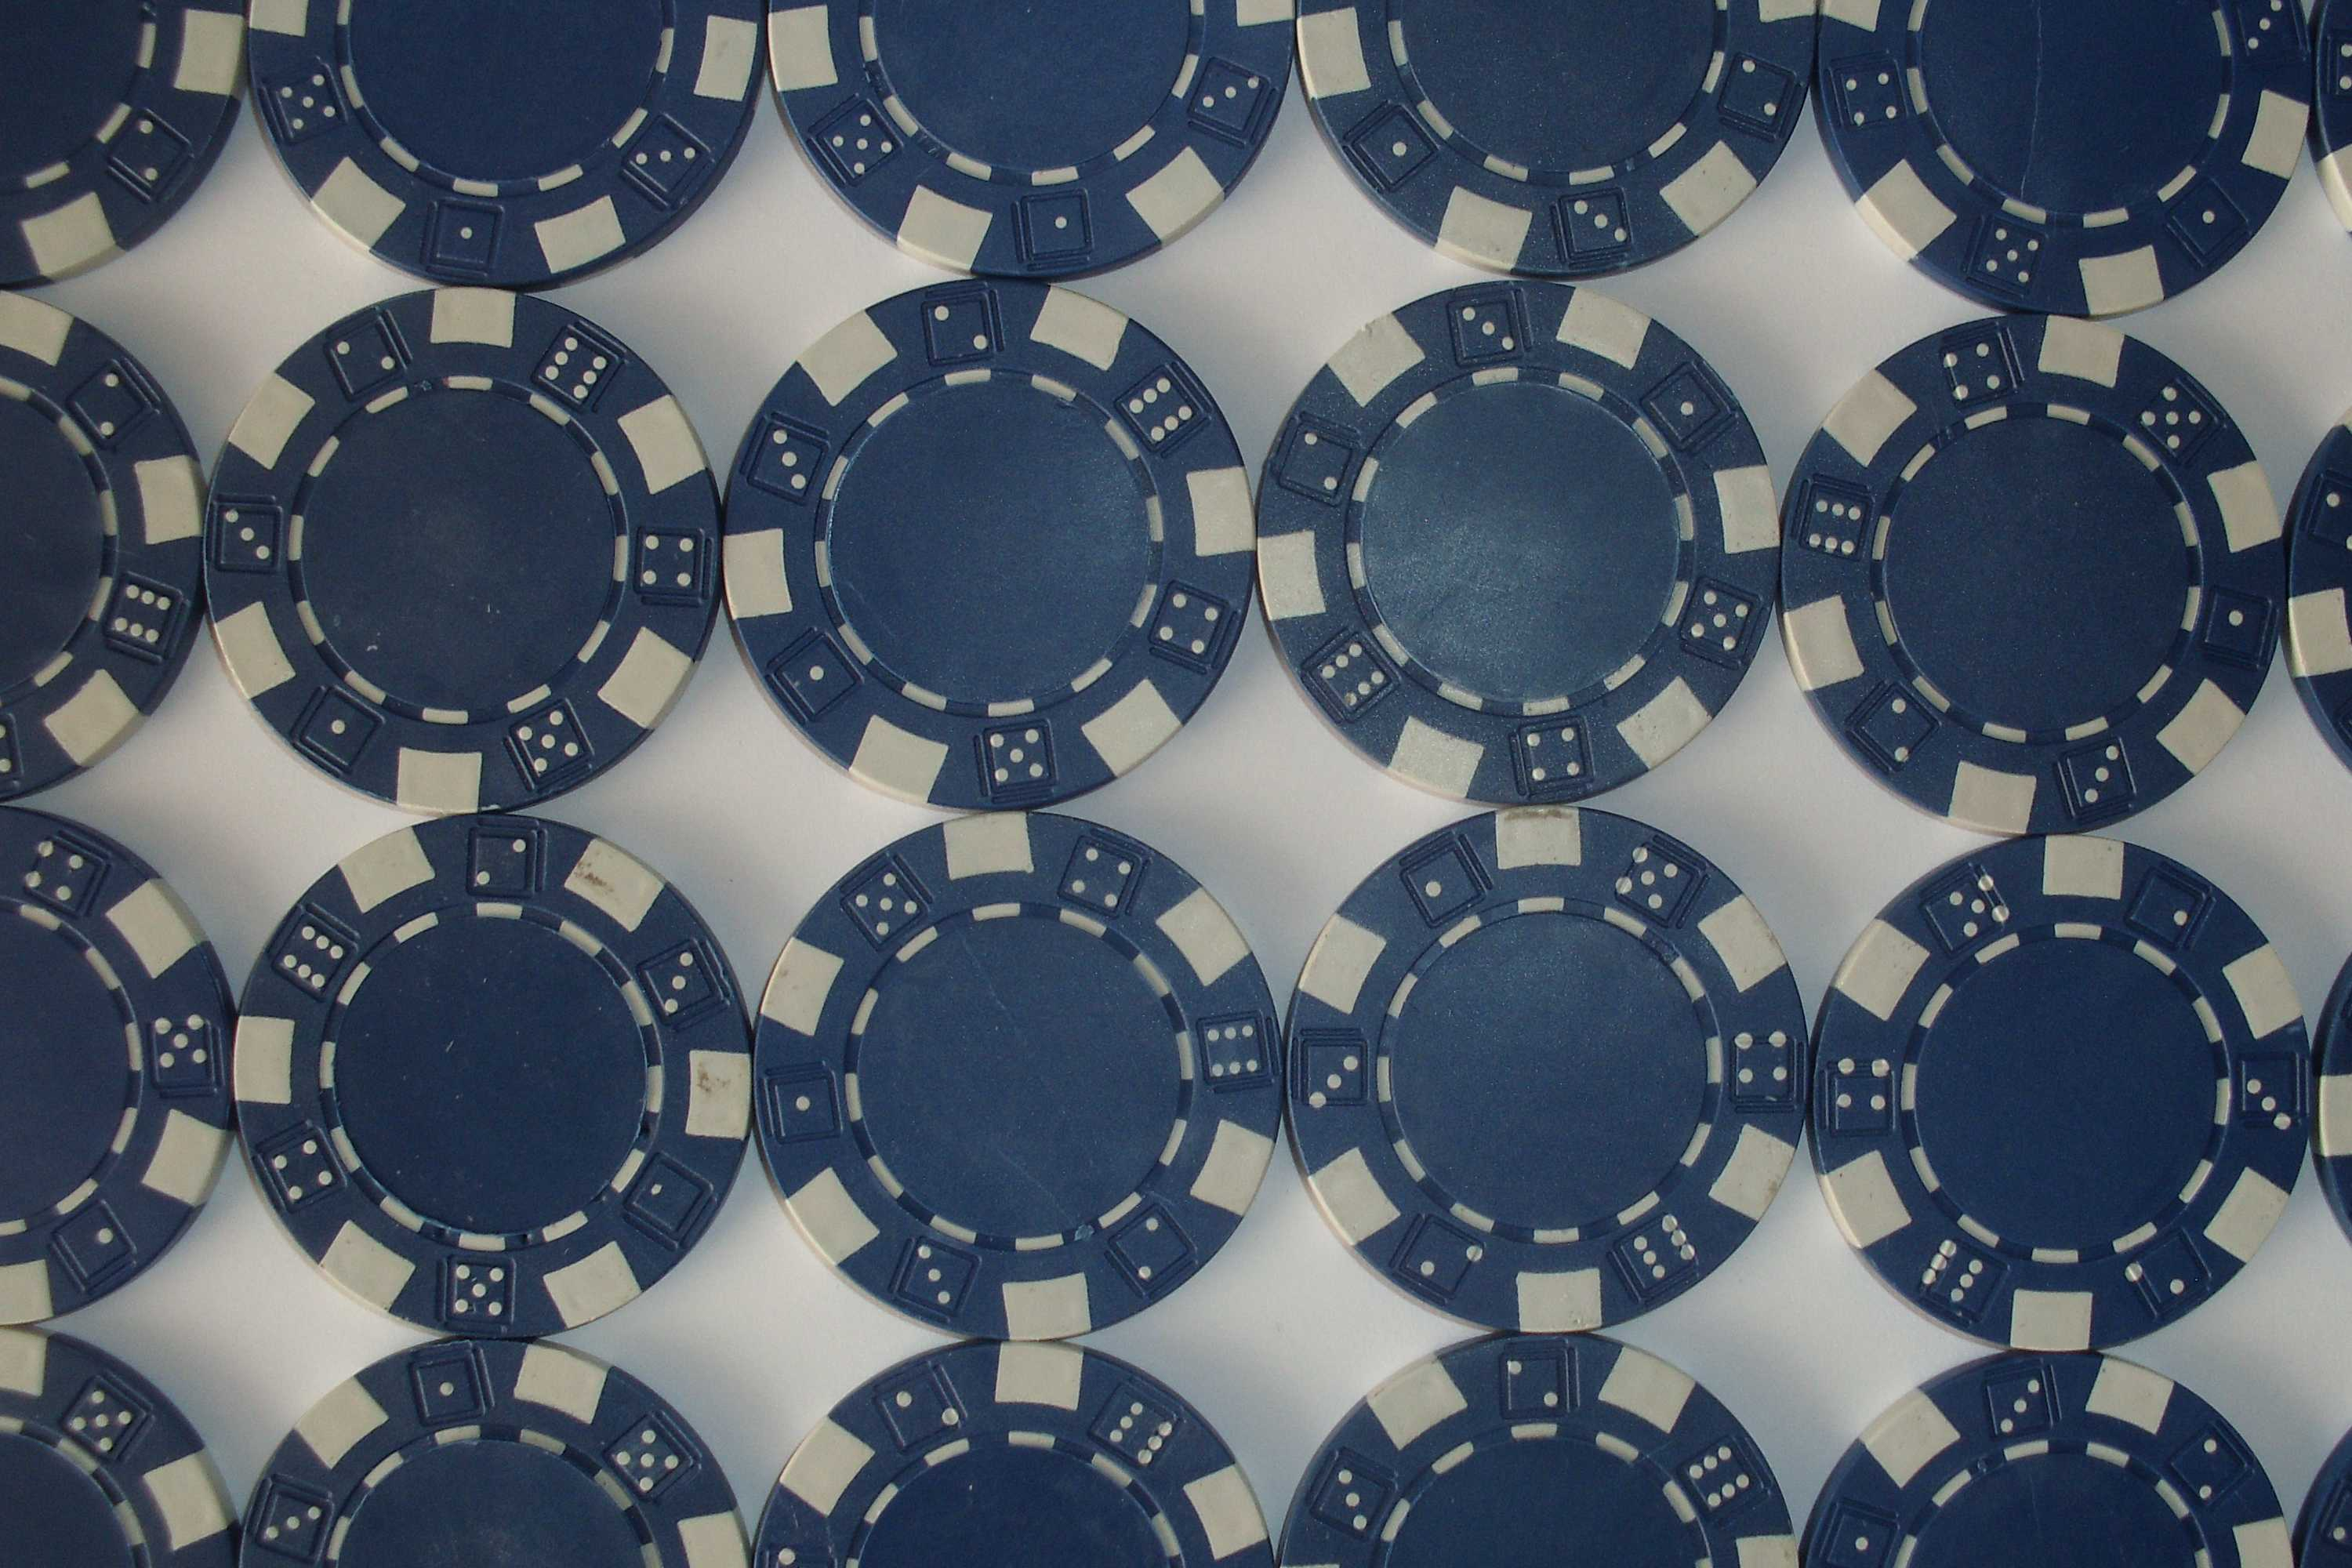
\includegraphics[height= 4cm]{jetons_sqr}\label{js}}\qquad
 % \subfloat[]{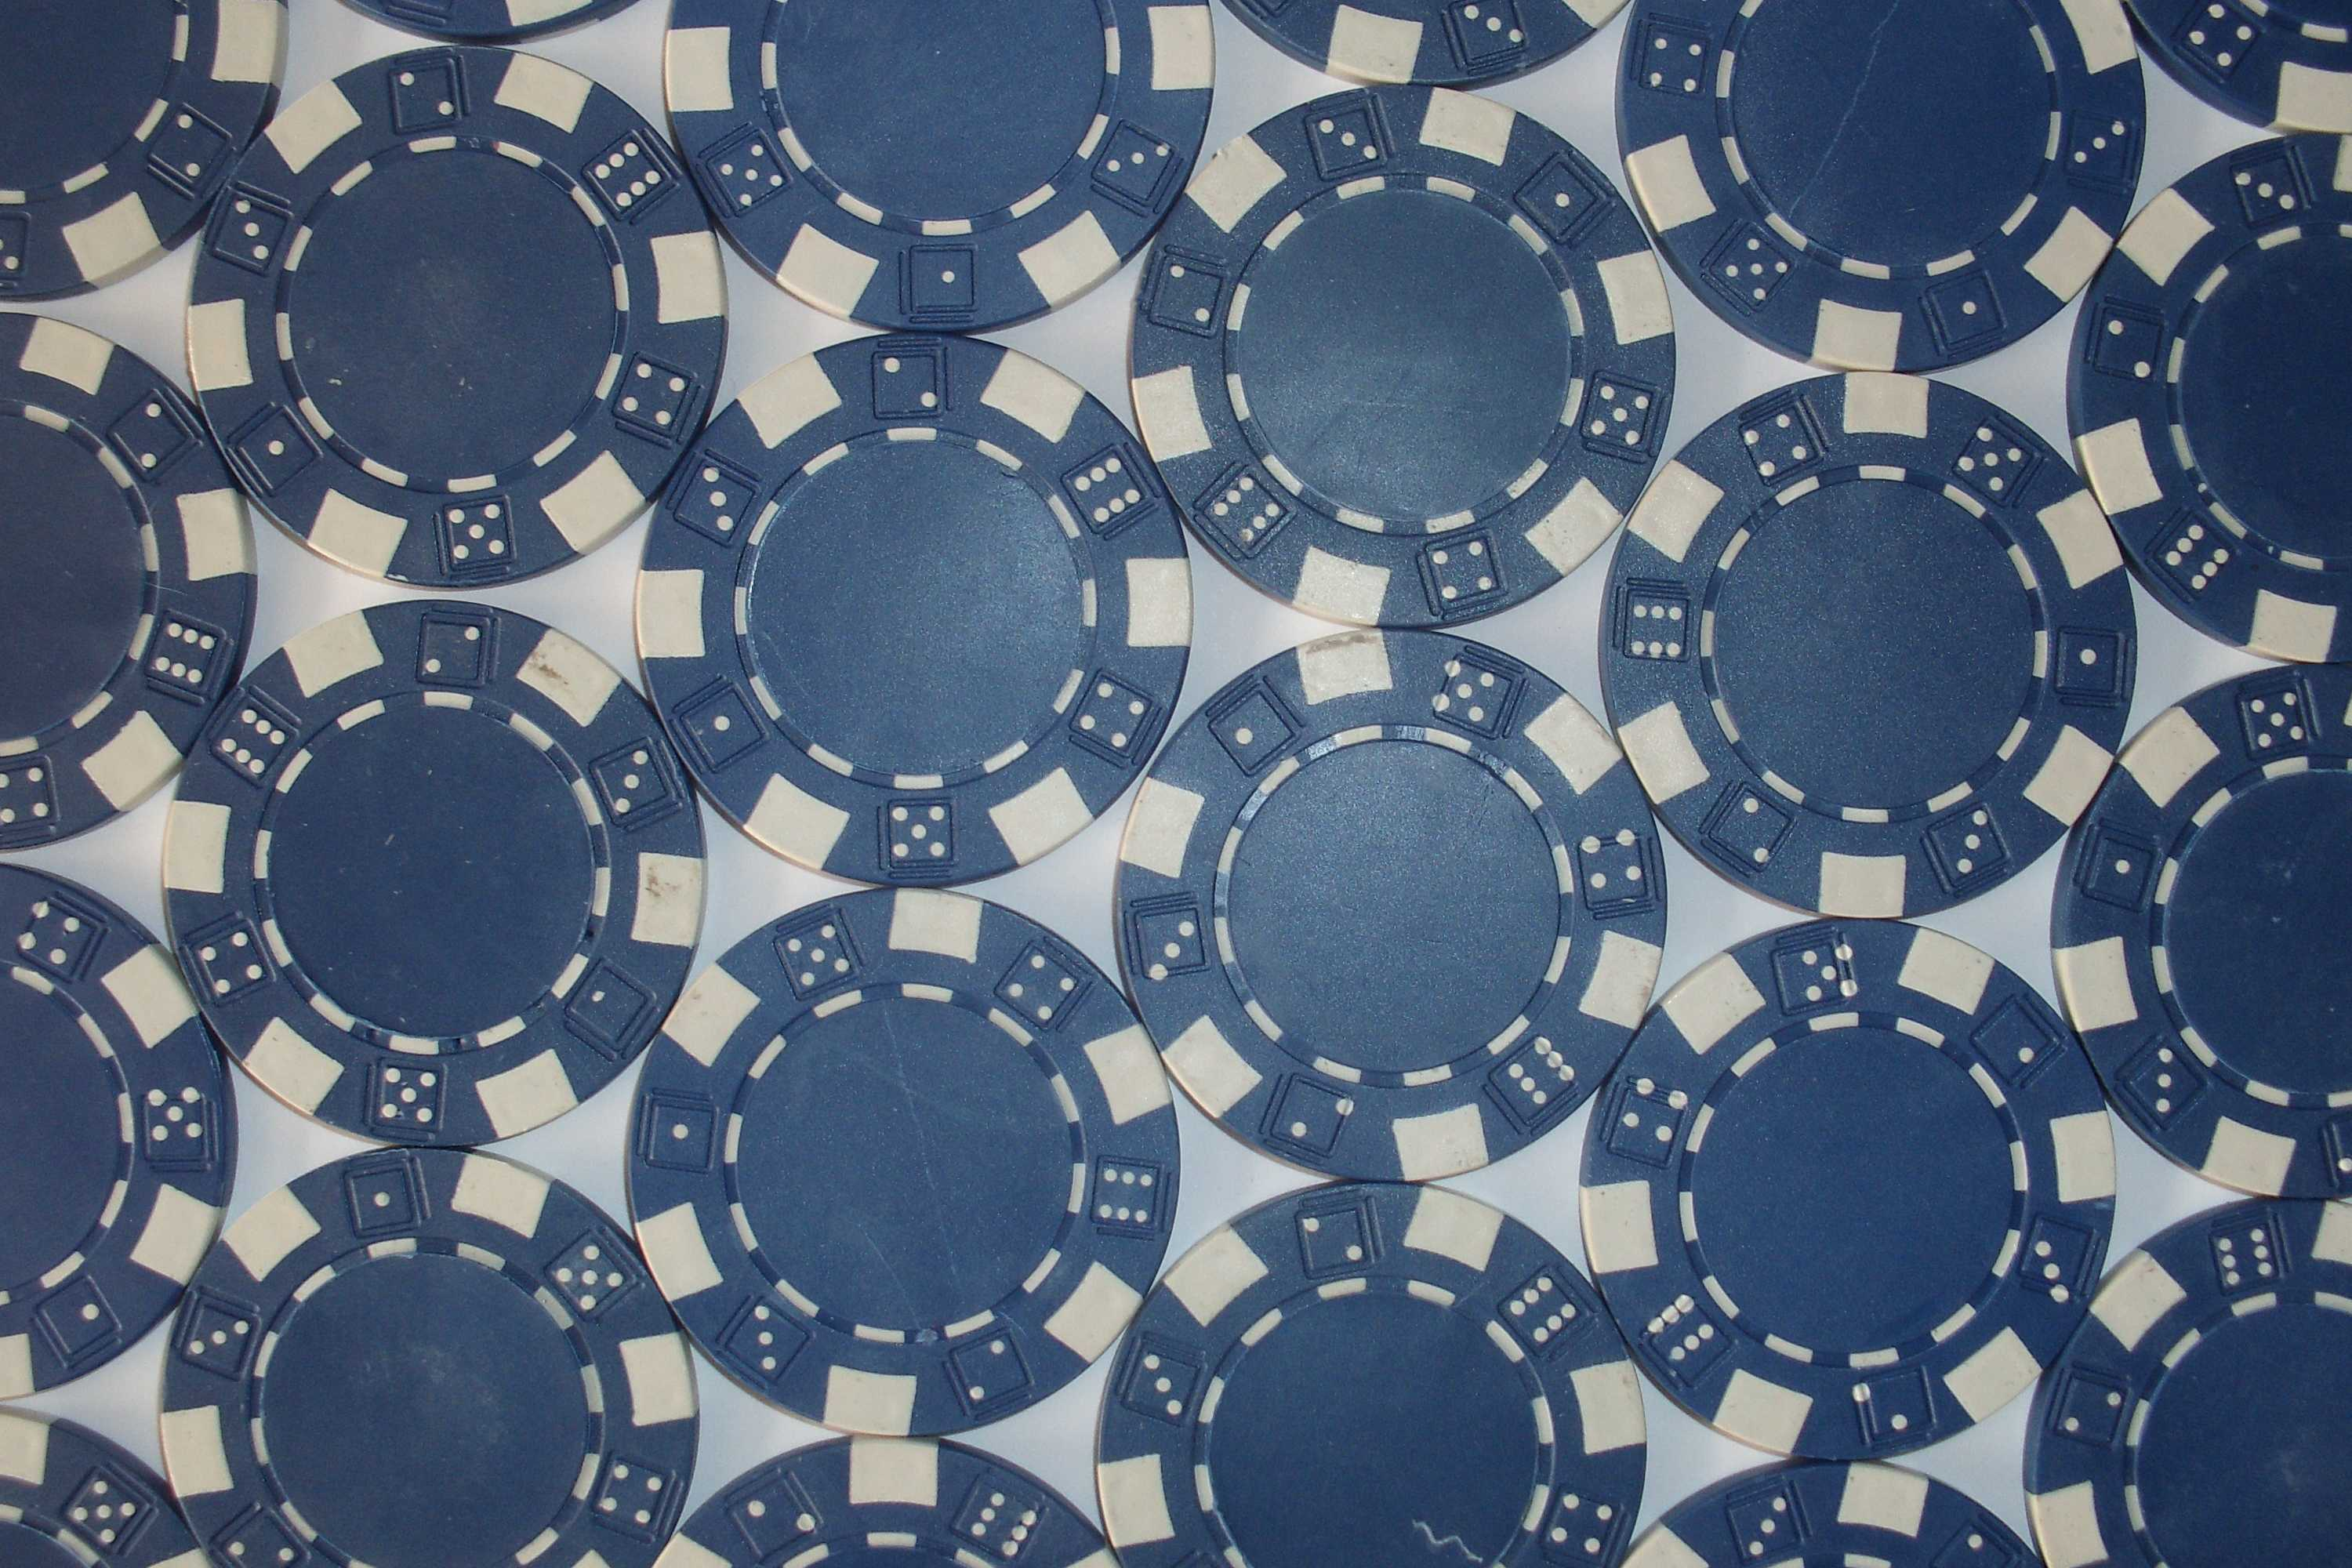
\includegraphics[height=4cm]{jetons_hex}\label{jh}}
 % \caption{Vierkante en hexagonale rangschikking met pokerjetons en hun voronoicellen.}  
%\end{figure}
\begin{columns}
        \begin{column}{0.4\textwidth}
    \begin{block}{Opdracht}
Probeer cirkels (munten, flippo's, pokerjetons ...) eens zodanig op een tafel te leggen dat er zo weinig mogelijk ruimte tussen de cirkels overblijft.
\end{block}
\end{column}
\begin{column}{0.4\textwidth}
      \only<2>{\begin{figure}[h]
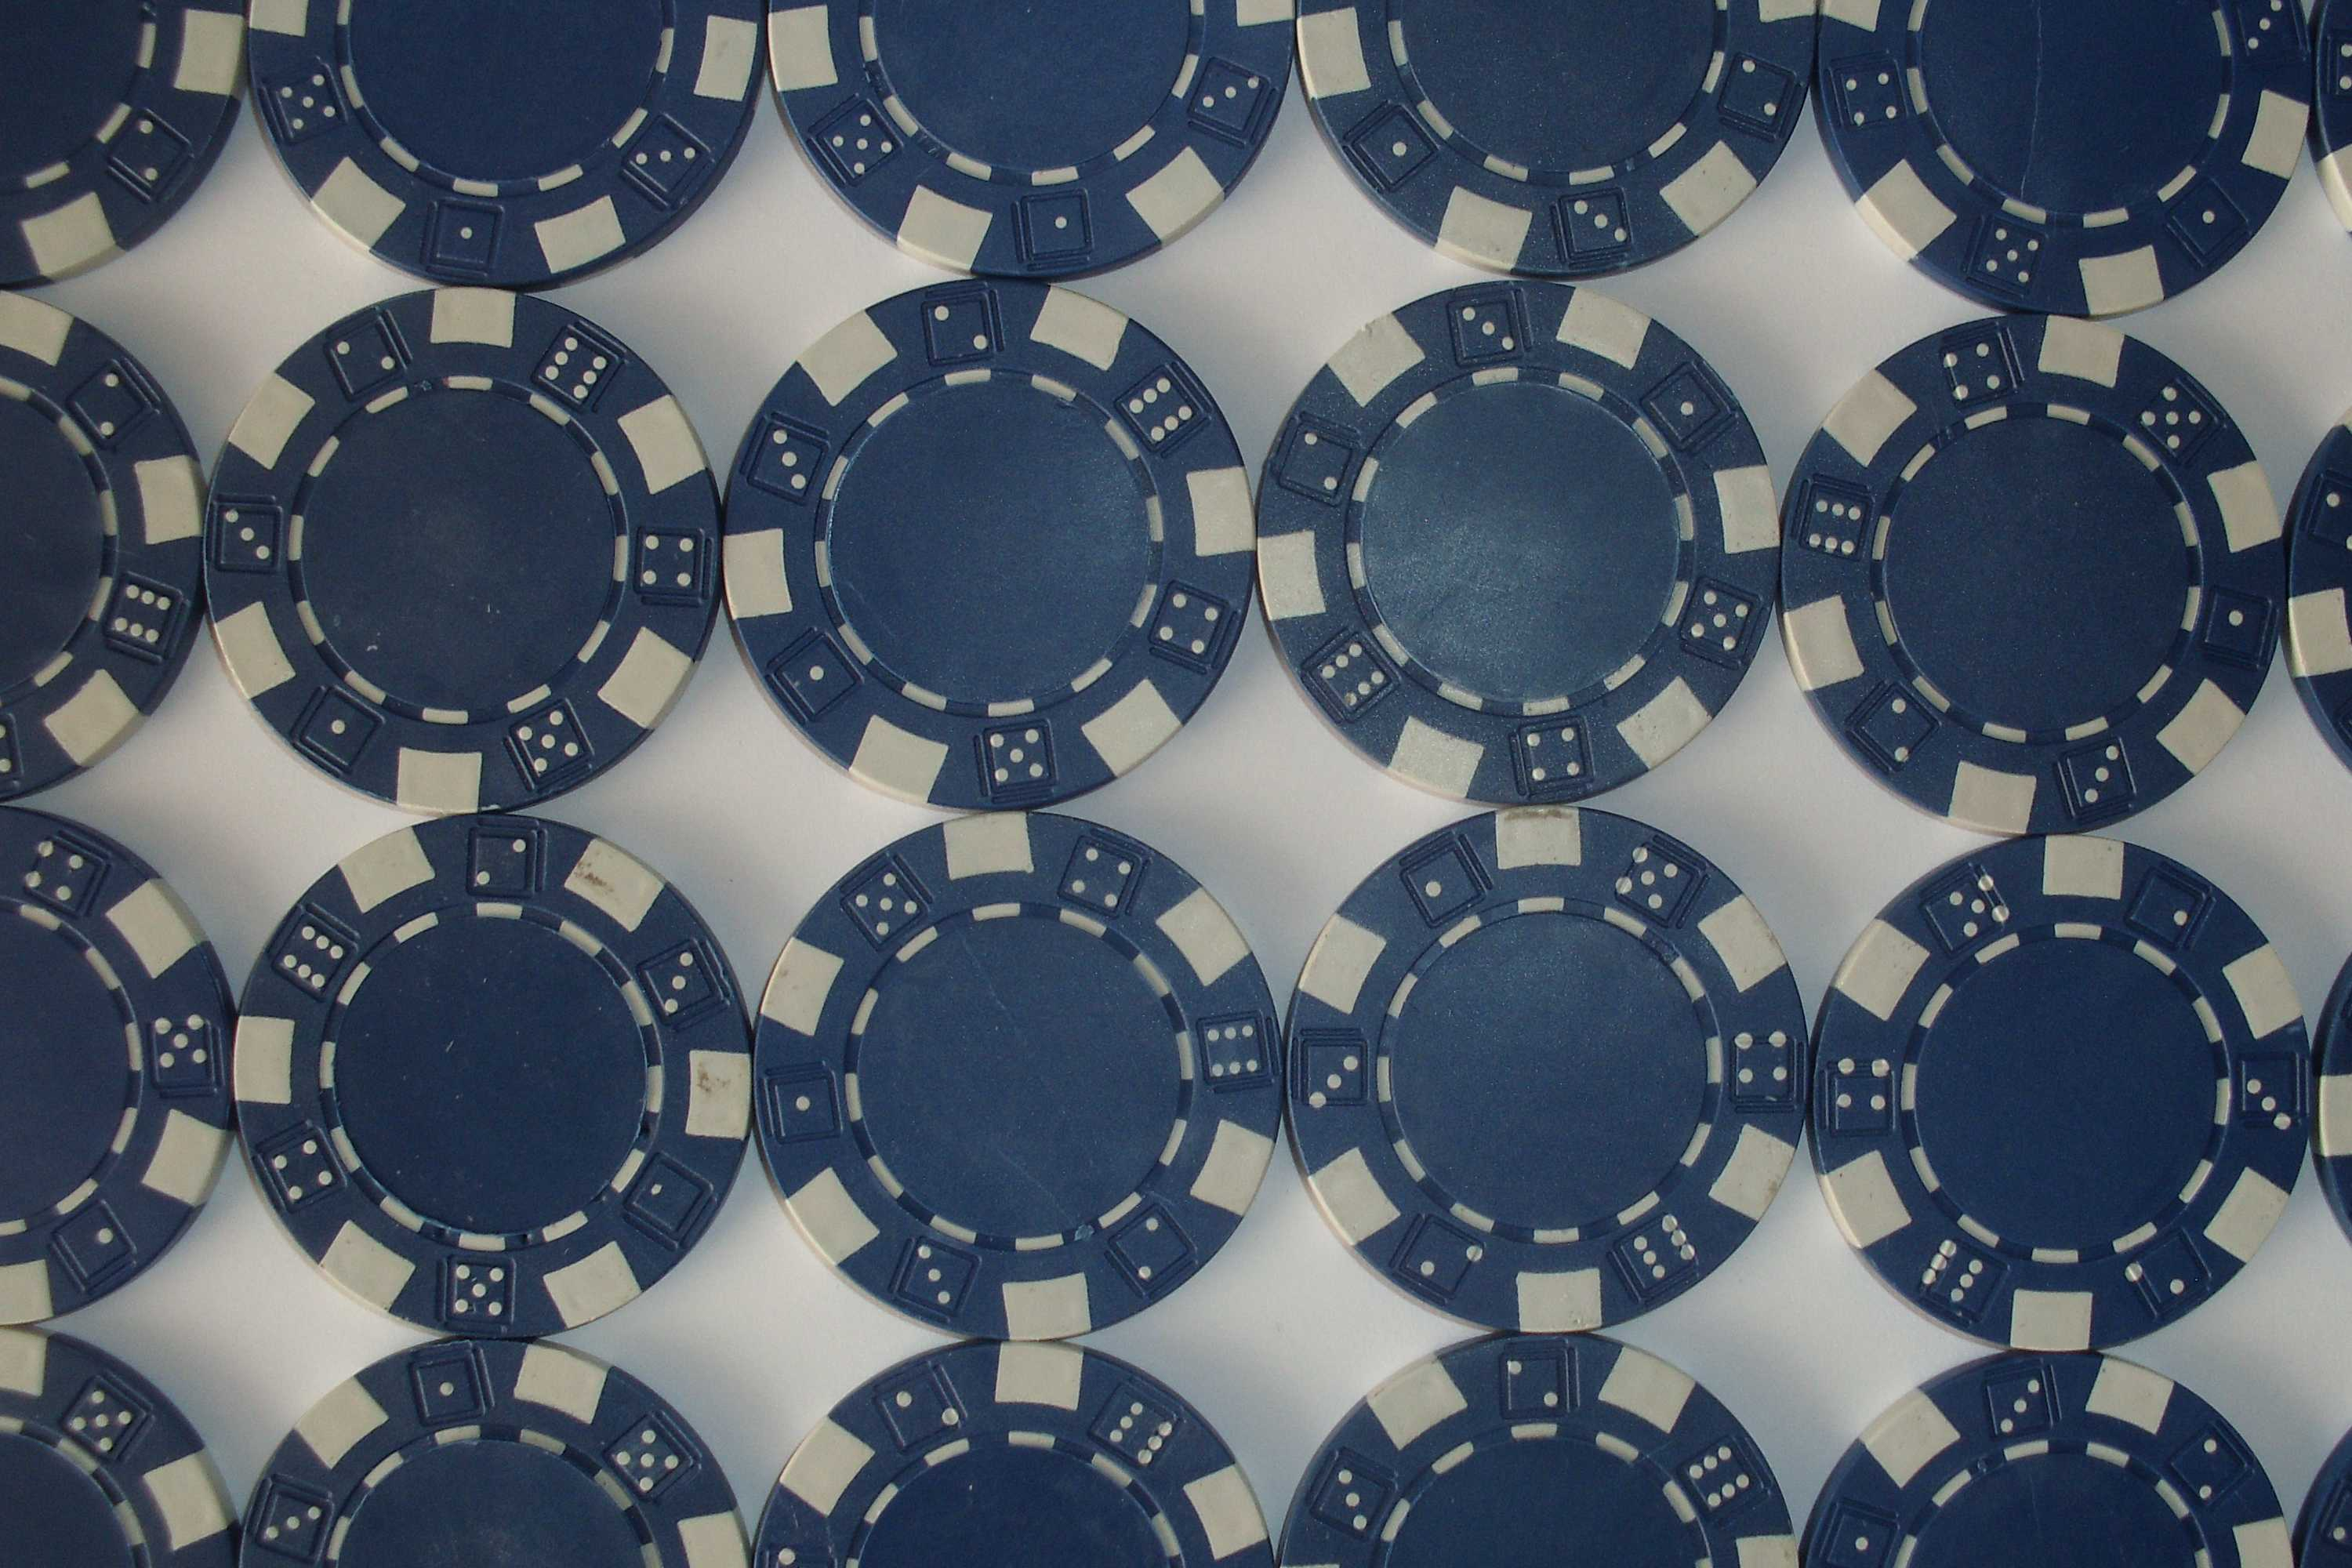
\includegraphics[width=\columnwidth]{jetons_sqr}
\end{figure}}
      \only<3>{\begin{figure}[h]
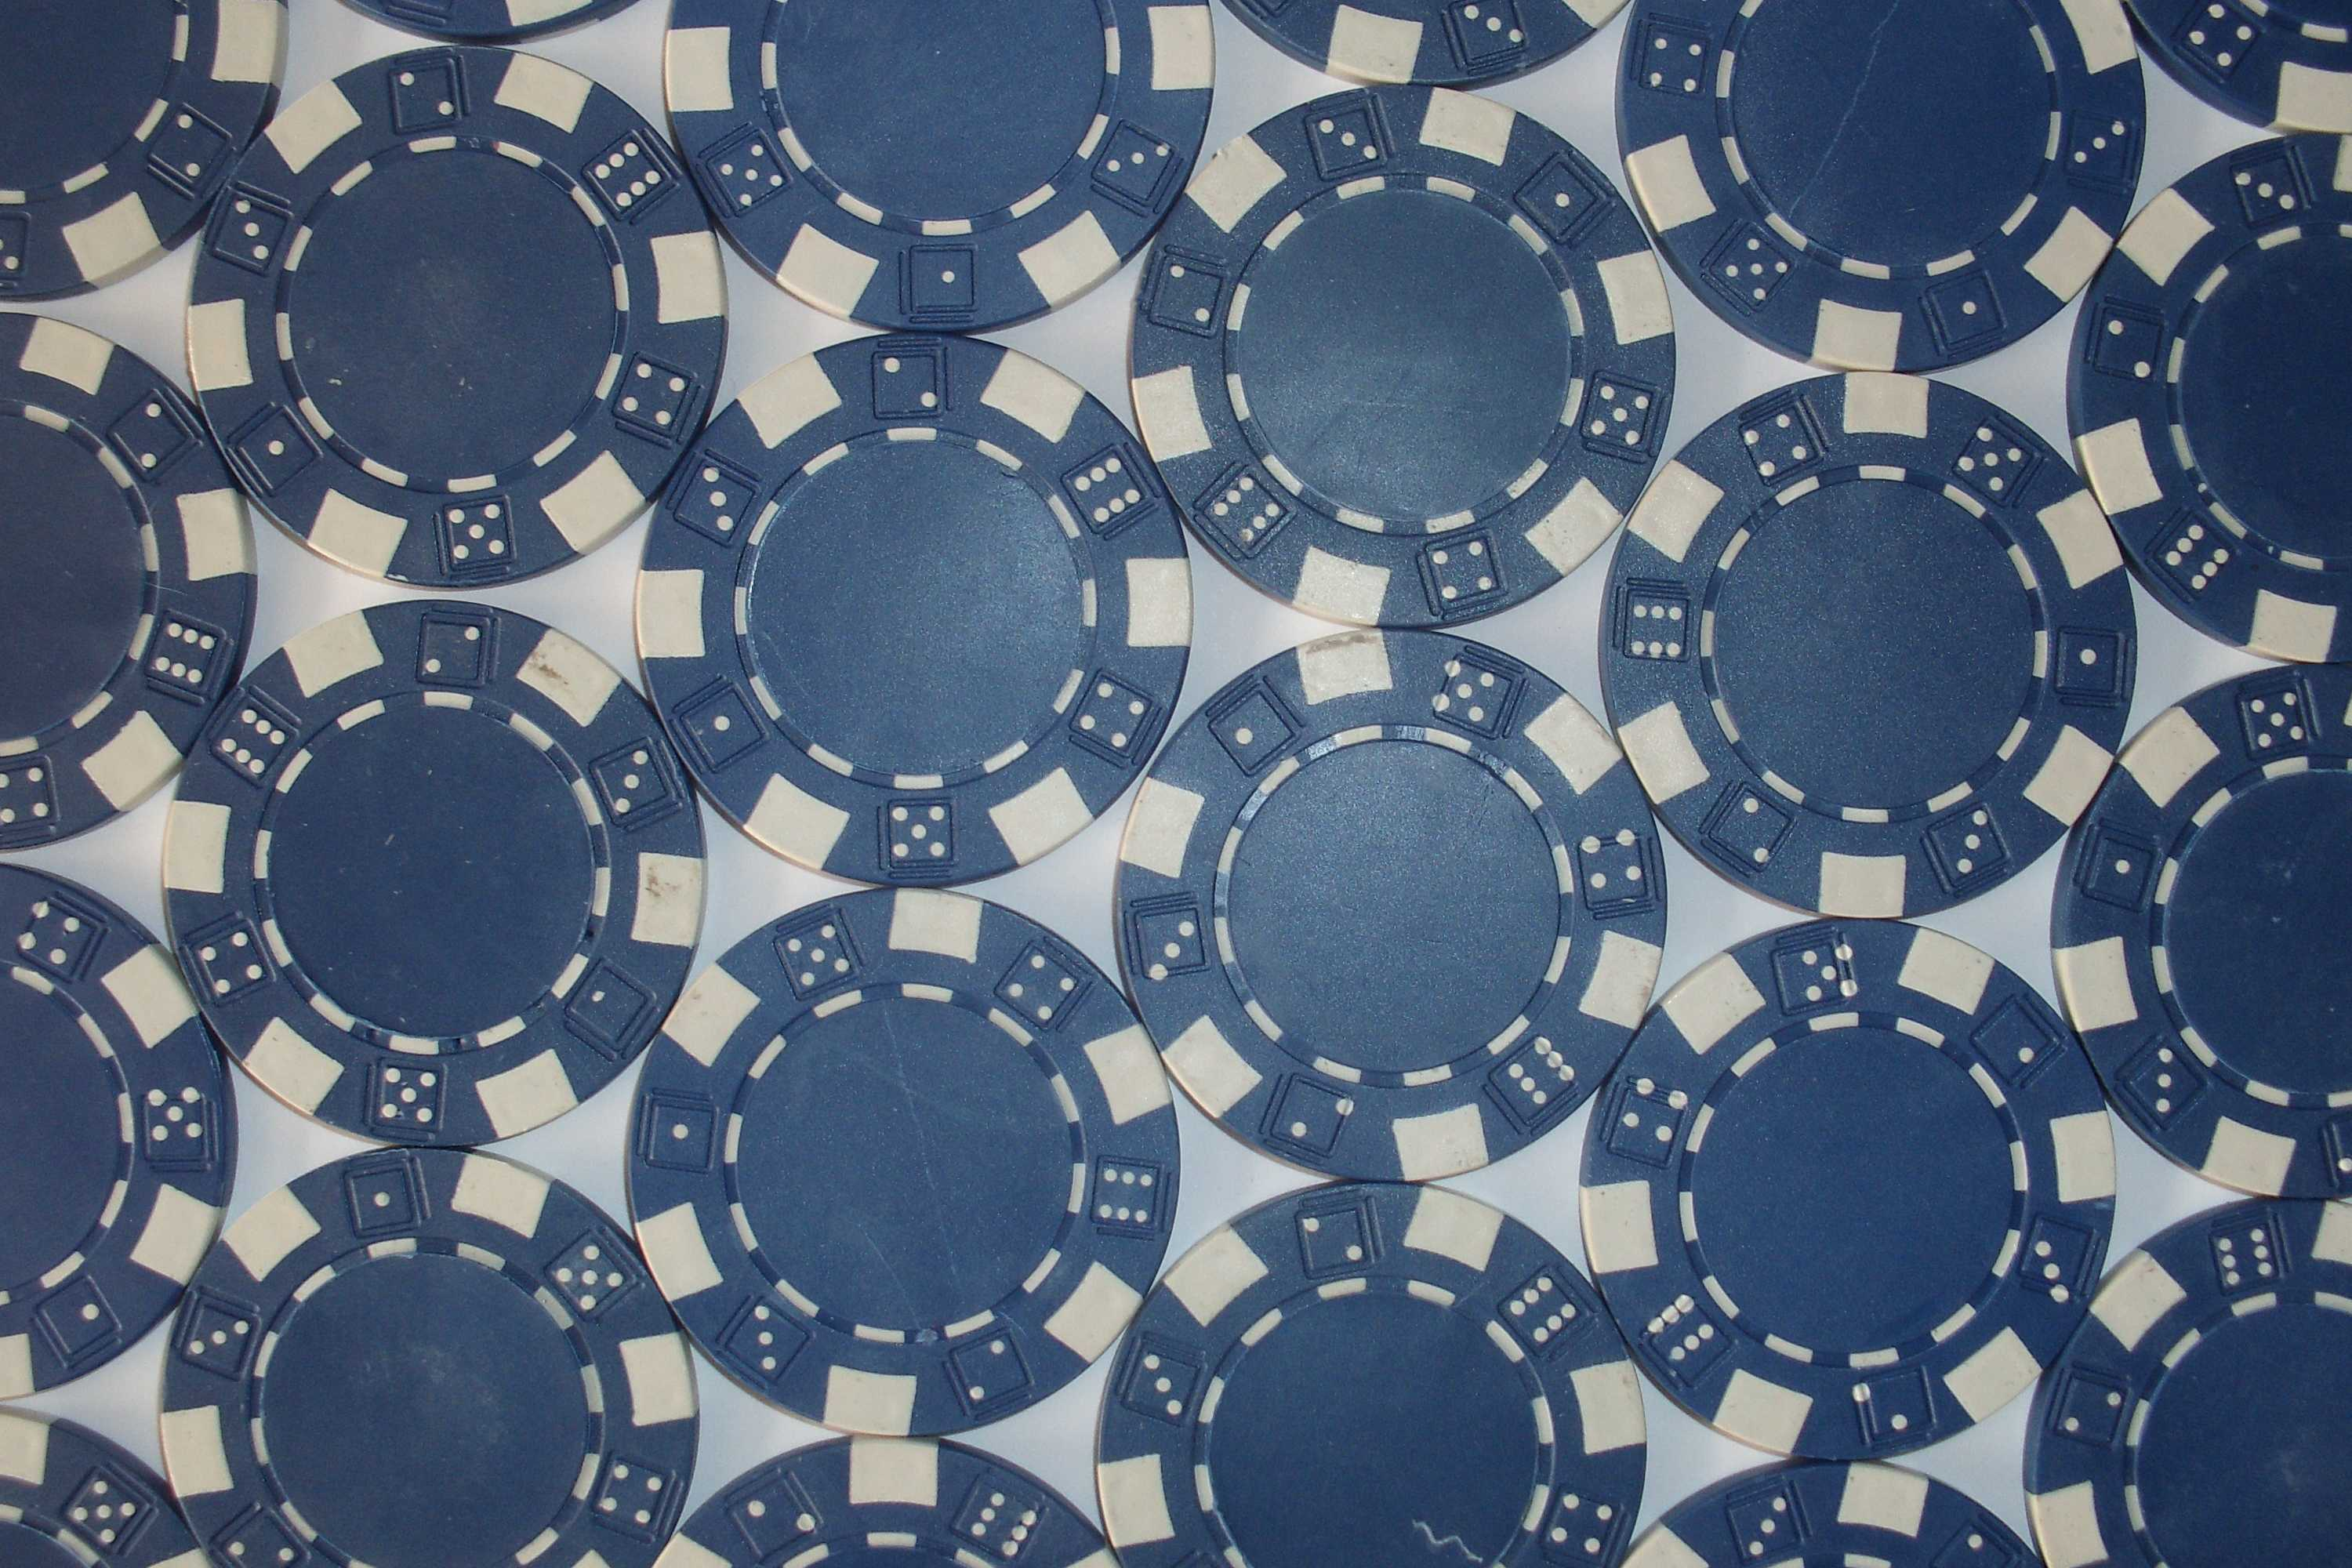
\includegraphics[width=\columnwidth]{jetons_hex}
\end{figure}}
    \end{column}
  \end{columns}  

\end{frame}

\begin{frame}\frametitle{Tweedimensionale stapelproblemen}
\begin{block}{Voronoicel}
De {\bf Voronoicel} van een cirkel is de verzameling van alle punten die dichter bij het middelpunt van deze cirkel liggen dan bij het middelpunt van elke andere cirkel in de schikking.
\end{block}
\end{frame}


\begin{frame}\frametitle{Tweedimensionale stapelproblemen}
\begin{block}{Voronoicel}
De {\bf Voronoicel} van een cirkel is de verzameling van alle punten die dichter bij het middelpunt van deze cirkel liggen dan bij het middelpunt van elke andere cirkel in de schikking.
\end{block}


\begin{block}{Vraag}
\begin{columns}

        \begin{column}{0.4\textwidth}
Hoe ziet de Voronoicel eruit bij een vierkante rangschikking? Hoe ziet de Voronoicel eruit bij de hexagonale rangschikking?\end{column}
\begin{column}{0.4\textwidth}
     
      \only<2>{\begin{figure}[h]
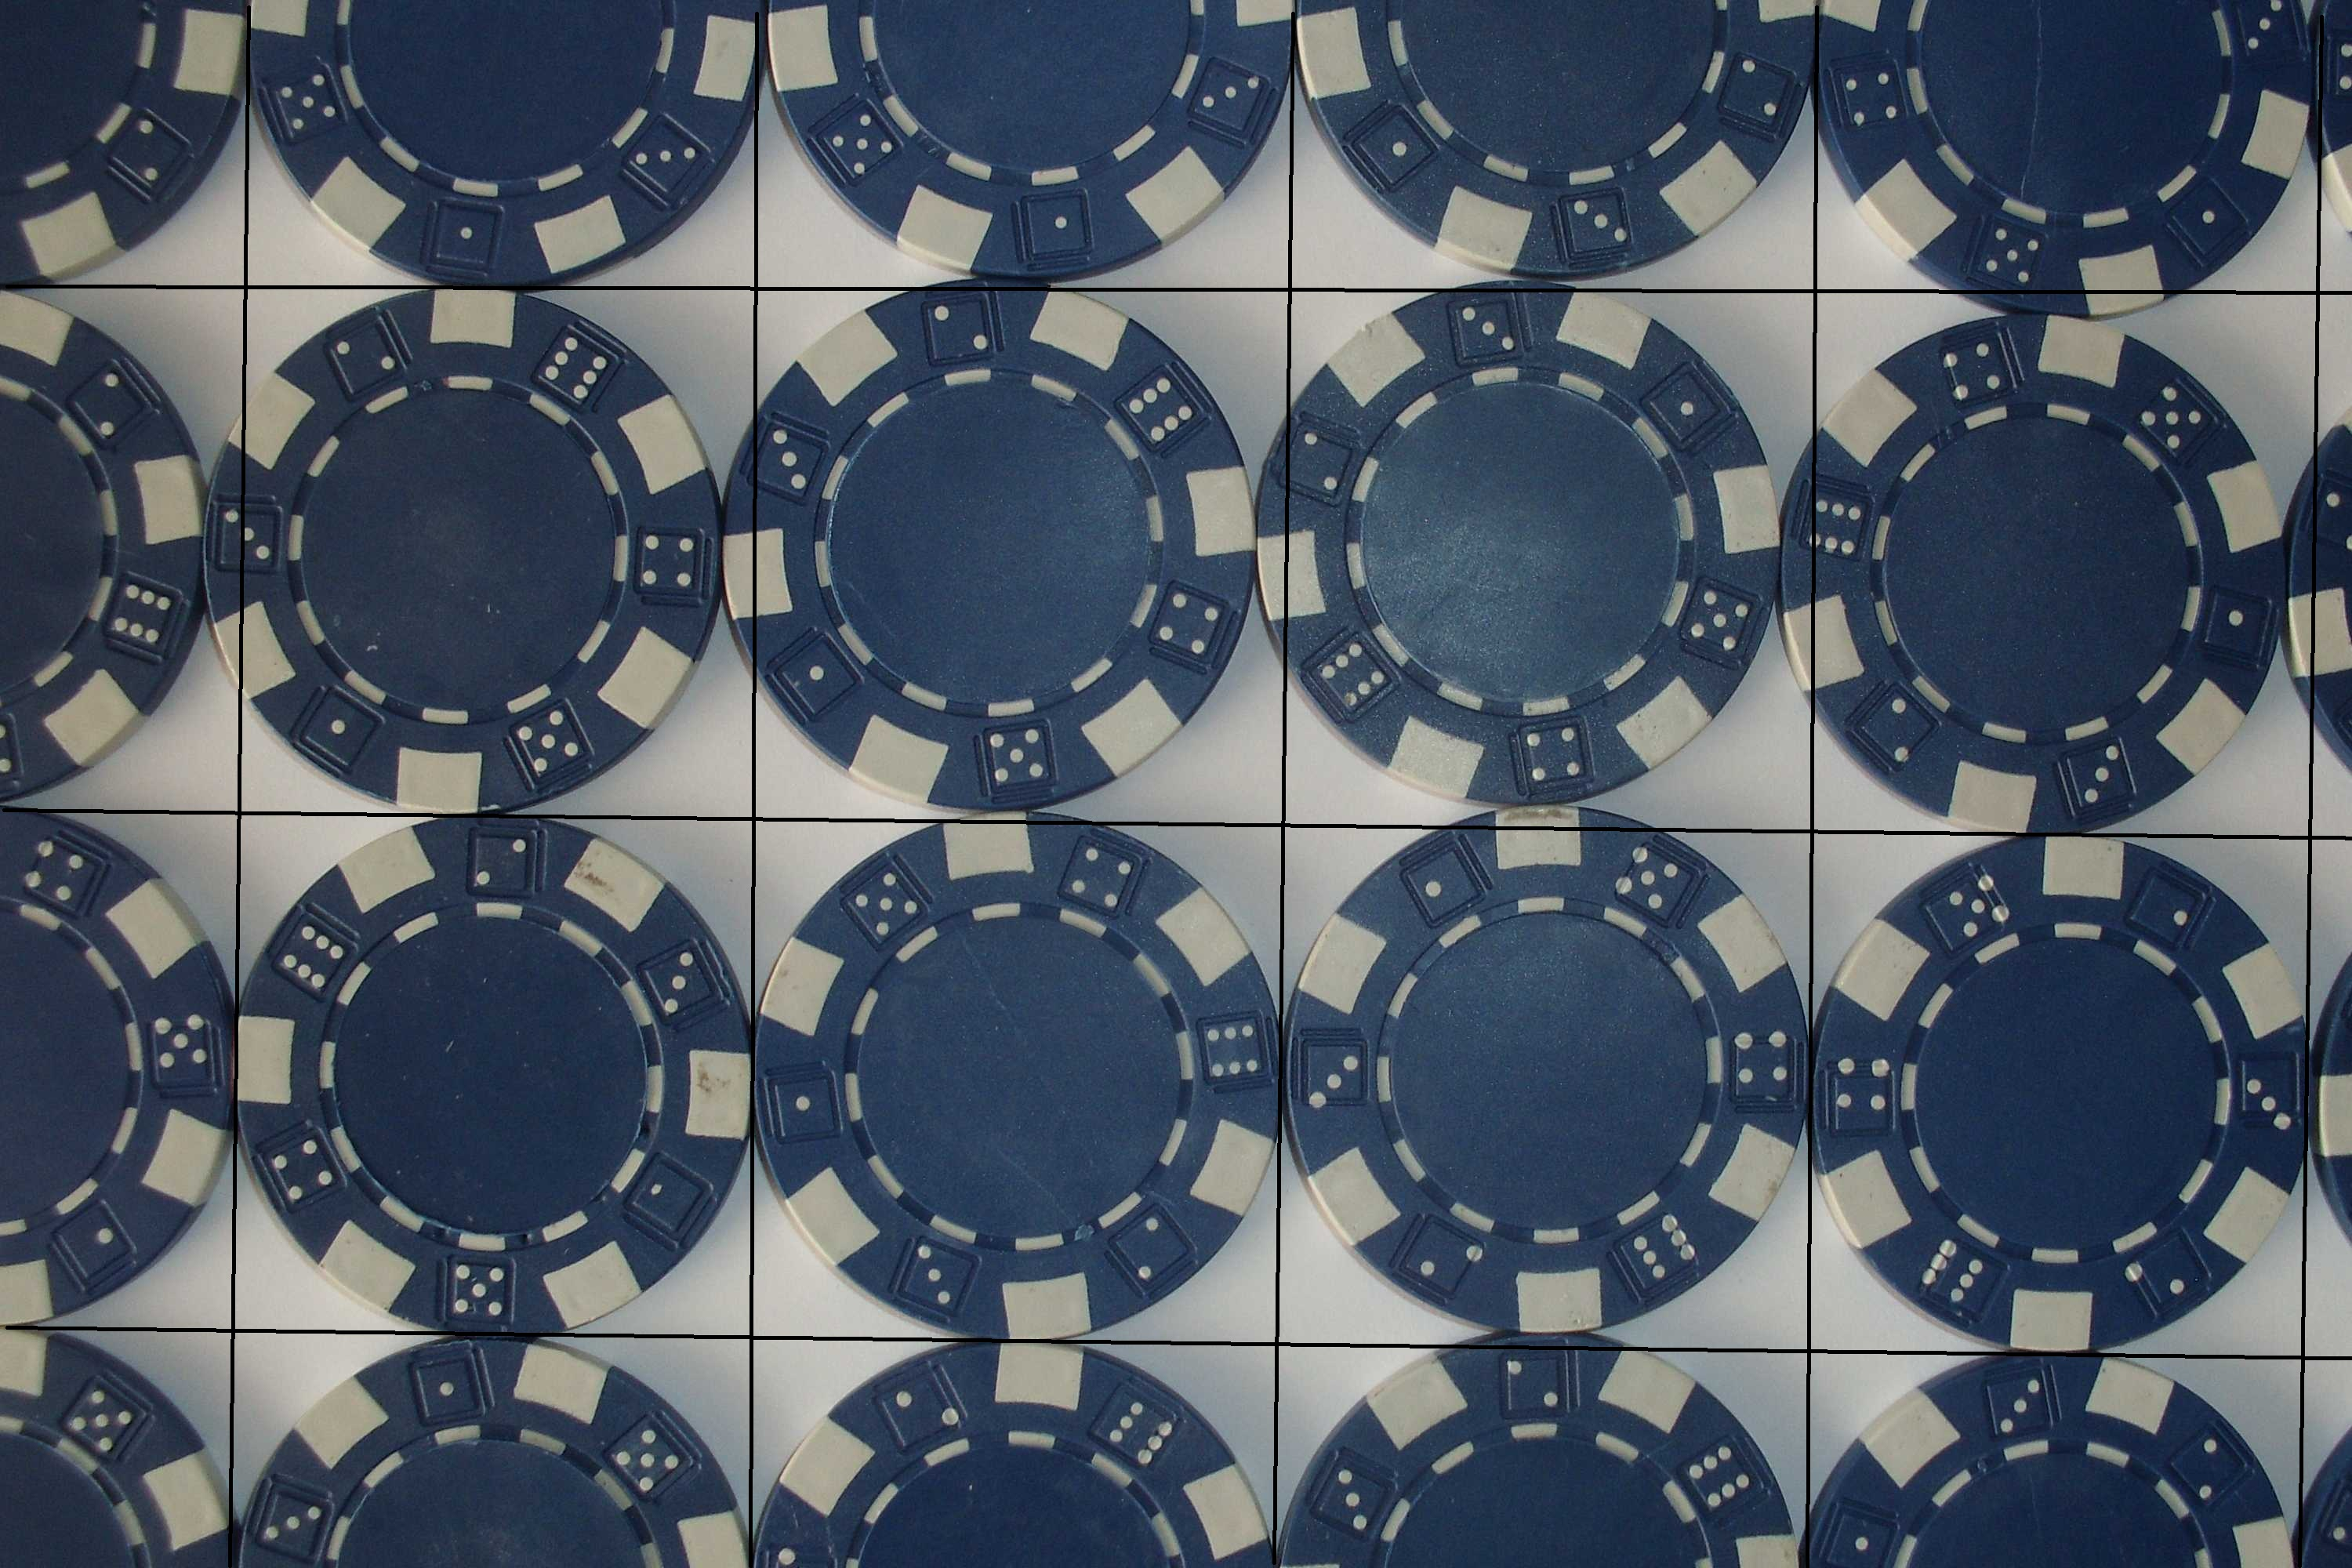
\includegraphics[width=\columnwidth]{voronoi_sqr}
\end{figure}}
      \only<3>{\begin{figure}[h]
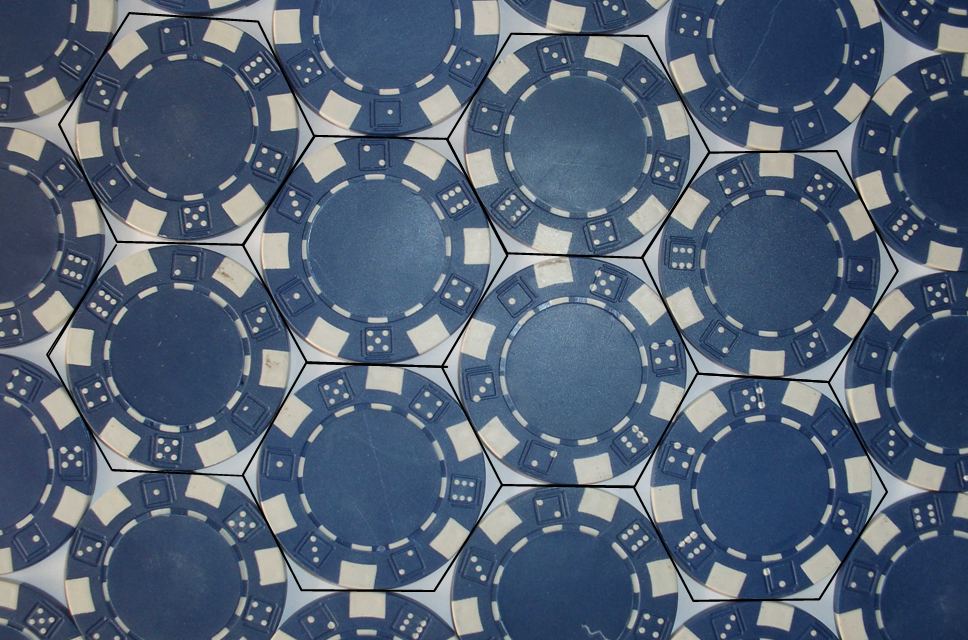
\includegraphics[width=\columnwidth]{voronoi_hex}
\end{figure}}

    \end{column}
  \end{columns}  
\end{block}%Omdat in het tweede deel van de les en ook de volgende les de leerlingen zelf de effici�ntie zullen moeten berekenen is het goed om dit al eens klassikaal te doen.
%\begin{block}{Vraag}
%Hoe kan je de effici�ntie berekenen aan de hand van zo'n Voronoicel?
%\end{block}
\end{frame}

\begin{frame}\frametitle{Tweedimensionale stapelproblemen}
\framesubtitle{Voronoicellen}
\begin{block}{Opdracht}
Bereken voor de vierkante en de hexagonale rangschikking de effici�ntie.
\end{block}
\pause
\begin{columns}
\begin{column}{0.6\textwidth}     
\begin{enumerate}
	\item Vierkante rangschikking: \\
 Effici�ntie = $\frac{\pi}{4}=0,78538...$
 \pause
	\item Hexagonale rangschikking:\\
	Effici�ntie = $\frac{\pi}{\sqrt{12}}=0.90689$
	%Dit is ook de meest effici�nte!!! -> Axel Thue heeft dit aangetoond en we geven in de cursus ook een kleine schets van het bewijs.
\end{enumerate}
\end{column}
\begin{column}{0.4\textwidth}     
     \begin{figure}[h]
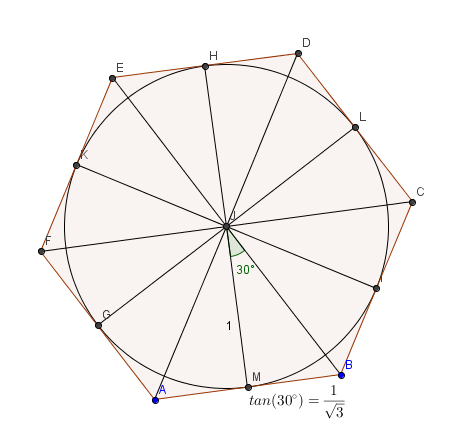
\includegraphics[width=\columnwidth]{hexagon}
\end{figure}
   \end{column}
\end{columns}  
\end{frame}

\begin{frame}
\frametitle{Tweedimensionale stapelproblemen}
\framesubtitle{Dienbladenprobleem: Opdracht}

Een fabrikant wil dienbladen voor een bepaalde aantal glazen of blikjes. Omdat de fabrikant ruimdenkend is, wil hij niet enkel de traditionele cirkelvormige dienbladen uitproberen, maar ook driehoekige, rechthoekige of zeshoekige dienbladen. 
\pause
\begin{block}{Opdracht}Bepaal nu voor een gegeven aantal glazen of blikjes we welk soort dienblad willen maken en wat juist de effici�ntie is%, m.a.w. hoeveel procent van het dienblad dat gevuld zal zijn
. Controleer dit voor dienbladen in de vorm van een cirkel, een gelijkzijdige driehoek, een rechthoek en een regelmatige zeshoek.
\end{block}
\end{frame}

\begin{frame}
\frametitle{Tweedimensionale stapelproblemen}
\framesubtitle{Dienbladenprobleem: Experimenteren}


\begin{table}[h]
\centering
\begin{tabular}{l||c|c|c|c}
Aantal / vorm & cirkelvormig & driehoekig & rechthoekig& zeshoekig\\\hline\hline
1&&&&\\\hline
2&&&&\\\hline
3&&&&\\\hline
4&&&&\\\hline
5&&&&\\\hline
6&&&&\\\hline
7&&&&\\\hline
8&&&&\\\hline
9&&&&\\\hline
10&&&&\\\hline
11&&&&\\\hline
12&&&&\\\hline
13&&&&\\\hline
...&&&&\\
\end{tabular}
\end{table}
\end{frame}



\begin{frame}
\frametitle{Tweedimensionale stapelproblemen}
\framesubtitle{Dienbladenprobleem: Experimenteren}

Hoe pakken we dit aan?

De klas wordt verdeeld in groepen die (al dan niet gesplitst)
\begin{enumerate}
	\item Experimenteren a.d.h.v. Geogebra-applets:
					\begin{itemize}
	          \item Cirkelvormig
	          \item Driehoekig
	          \item Rechthoekig
	          \item Zeshoekig	          
          \end{itemize}
	
	\item Experimenteren a.d.h.v. pokerjetons, karton en liniaal:
		\begin{itemize}
	\item Driehoekig
	\item Rechthoekig
\end{itemize}
	\end{enumerate}

\end{frame}


\begin{frame}
\frametitle{Tweedimensionale stapelproblemen}
\framesubtitle{Dienbladenprobleem: Experimenteren en berekenen}

\begin{figure}[h]
\centering
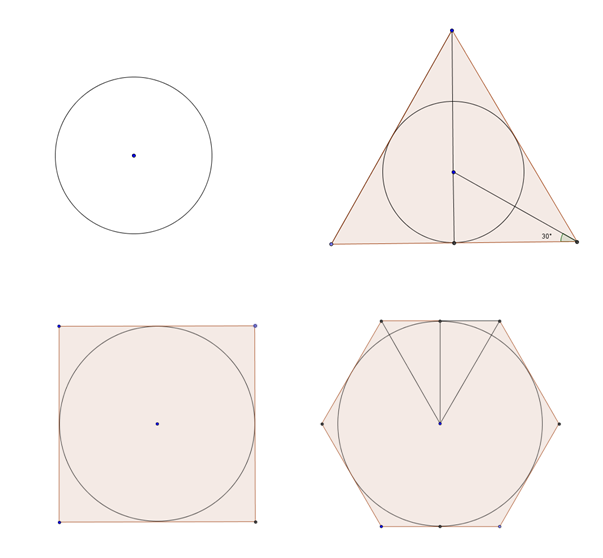
\includegraphics[height=5cm]{1munten}
\caption{De dienbladen voor 1 munt.}
\label{2munt}
\end{figure}

\end{frame}


\begin{frame}
\frametitle{Tweedimensionale stapelproblemen}
\framesubtitle{Dienbladenprobleem: Experimenteren en berekenen}

\begin{figure}[h]
\centering
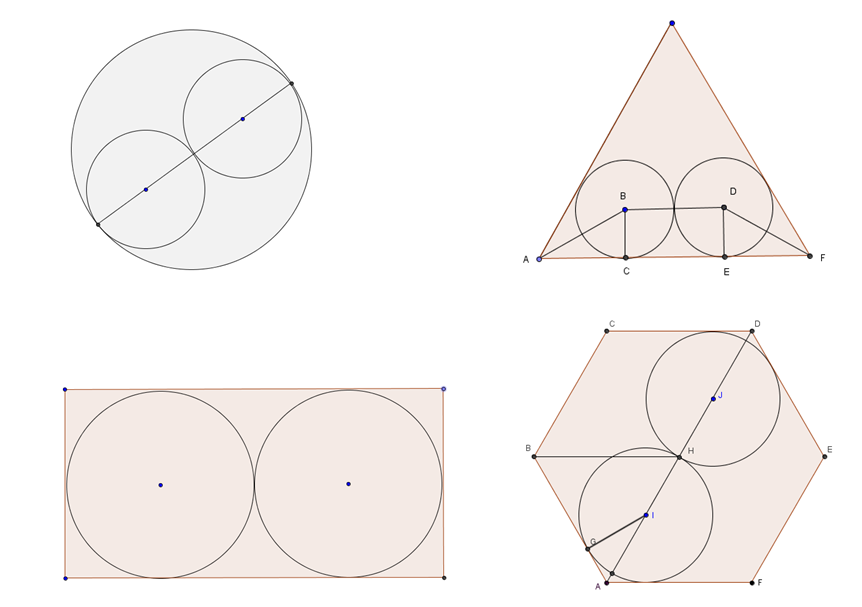
\includegraphics[height=5cm]{2munten}
\caption{De dienbladen voor 2 munten.}
\label{2munt}
\end{figure}

\end{frame}


\begin{frame}
\frametitle{Tweedimensionale stapelproblemen}
\framesubtitle{Dienbladenprobleem: Experimenteren en berekenen}

\begin{figure}[h]
\centering
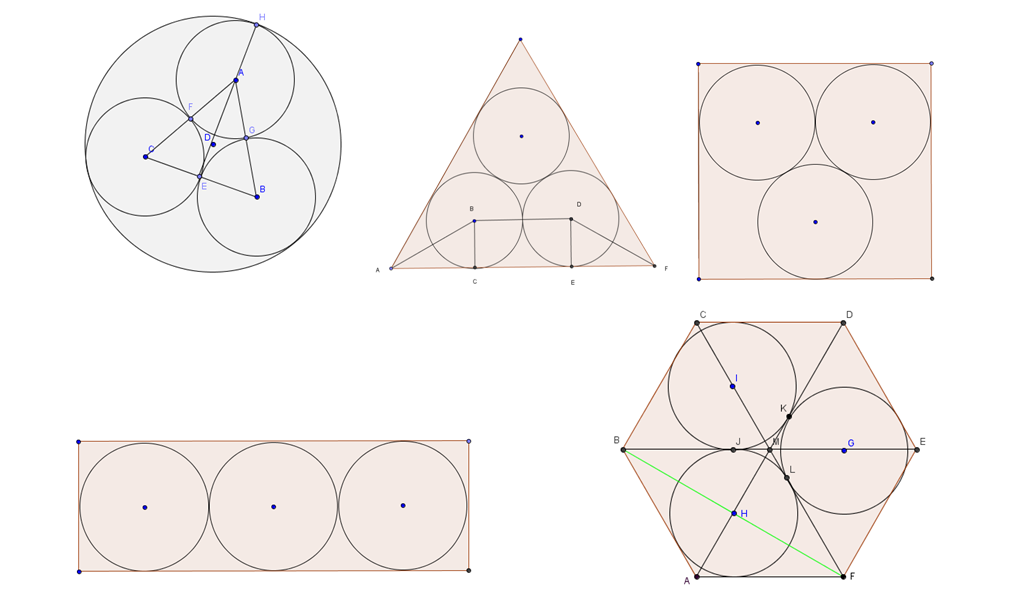
\includegraphics[height=5cm]{3munten}
\caption{De dienbladen voor 3 munten.}
\label{2munt}
\end{figure}

\end{frame}
